% REV01 Tue 22 Jun 2021 17:10:07 WIB
% START Tue 04 May 2021 13:55:16 WIB

\chapter{STILL EDUCATIONAL}

The person of the house, doll’s dressmaker and manufacturer of
ornamental pincushions and pen-wipers, sat in her quaint little low
arm-chair, singing in the dark, until Lizzie came back. The person
of the house had attained that dignity while yet of very tender years
indeed, through being the only trustworthy person IN the house.

‘Well Lizzie-Mizzie-Wizzie,’ said she, breaking off in her song, ‘what’s
the news out of doors?’

‘What’s the news in doors?’ returned Lizzie, playfully smoothing the
bright long fair hair which grew very luxuriant and beautiful on the
head of the doll’s dressmaker.

‘Let me see, said the blind man. Why the last news is, that I don’t mean
to marry your brother.’

‘No?’

‘No-o,’ shaking her head and her chin. ‘Don’t like the boy.’

‘What do you say to his master?’

‘I say that I think he’s bespoke.’

Lizzie finished putting the hair carefully back over the misshapen
shoulders, and then lighted a candle. It showed the little parlour to
be dingy, but orderly and clean. She stood it on the mantelshelf, remote
from the dressmaker’s eyes, and then put the room door open, and the
house door open, and turned the little low chair and its occupant
towards the outer air. It was a sultry night, and this was a
fine-weather arrangement when the day’s work was done. To complete
it, she seated herself in a chair by the side of the little chair, and
protectingly drew under her arm the spare hand that crept up to her.

‘This is what your loving Jenny Wren calls the best time in the day and
night,’ said the person of the house. Her real name was Fanny Cleaver;
but she had long ago chosen to bestow upon herself the appellation of
Miss Jenny Wren.

‘I have been thinking,’ Jenny went on, ‘as I sat at work to-day, what
a thing it would be, if I should be able to have your company till I am
married, or at least courted. Because when I am courted, I shall make
Him do some of the things that you do for me. He couldn’t brush my hair
like you do, or help me up and down stairs like you do, and he couldn’t
do anything like you do; but he could take my work home, and he could
call for orders in his clumsy way. And he shall too. I’LL trot him
about, I can tell him!’

Jenny Wren had her personal vanities--happily for her--and no intentions
were stronger in her breast than the various trials and torments that
were, in the fulness of time, to be inflicted upon ‘him.’

‘Wherever he may happen to be just at present, or whoever he may happen
to be,’ said Miss Wren, ‘I know his tricks and his manners, and I give
him warning to look out.’

‘Don’t you think you are rather hard upon him?’ asked her friend,
smiling, and smoothing her hair.

‘Not a bit,’ replied the sage Miss Wren, with an air of vast experience.
‘My dear, they don’t care for you, those fellows, if you’re NOT hard
upon ‘em. But I was saying If I should be able to have your company. Ah!
What a large If! Ain’t it?’

‘I have no intention of parting company, Jenny.’

‘Don’t say that, or you’ll go directly.’

‘Am I so little to be relied upon?’

‘You’re more to be relied upon than silver and gold.’ As she said it,
Miss Wren suddenly broke off, screwed up her eyes and her chin, and
looked prodigiously knowing. ‘Aha!

\begin{verbatim}
     Who comes here?
     A Grenadier.
     What does he want?
     A pot of beer.
\end{verbatim}

And nothing else in the world, my dear!’

A man’s figure paused on the pavement at the outer door. ‘Mr Eugene
Wrayburn, ain’t it?’ said Miss Wren.

‘So I am told,’ was the answer.

‘You may come in, if you’re good.’

‘I am not good,’ said Eugene, ‘but I’ll come in.’

He gave his hand to Jenny Wren, and he gave his hand to Lizzie, and he
stood leaning by the door at Lizzie’s side. He had been strolling with
his cigar, he said, (it was smoked out and gone by this time,) and he
had strolled round to return in that direction that he might look in as
he passed. Had she not seen her brother to-night?

‘Yes,’ said Lizzie, whose manner was a little troubled.

Gracious condescension on our brother’s part! Mr Eugene Wrayburn thought
he had passed my young gentleman on the bridge yonder. Who was his
friend with him?

‘The schoolmaster.’

‘To be sure. Looked like it.’

Lizzie sat so still, that one could not have said wherein the fact of
her manner being troubled was expressed; and yet one could not have
doubted it. Eugene was as easy as ever; but perhaps, as she sat with
her eyes cast down, it might have been rather more perceptible that
his attention was concentrated upon her for certain moments, than its
concentration upon any subject for any short time ever was, elsewhere.

‘I have nothing to report, Lizzie,’ said Eugene. ‘But, having promised
you that an eye should be always kept on Mr Riderhood through my friend
Lightwood, I like occasionally to renew my assurance that I keep my
promise, and keep my friend up to the mark.’

‘I should not have doubted it, sir.’

‘Generally, I confess myself a man to be doubted,’ returned Eugene,
coolly, ‘for all that.’

‘Why are you?’ asked the sharp Miss Wren.

‘Because, my dear,’ said the airy Eugene, ‘I am a bad idle dog.’

‘Then why don’t you reform and be a good dog?’ inquired Miss Wren.

‘Because, my dear,’ returned Eugene, ‘there’s nobody who makes it worth
my while. Have you considered my suggestion, Lizzie?’ This in a lower
voice, but only as if it were a graver matter; not at all to the
exclusion of the person of the house.

‘I have thought of it, Mr Wrayburn, but I have not been able to make up
my mind to accept it.’

‘False pride!’ said Eugene.

‘I think not, Mr Wrayburn. I hope not.’

‘False pride!’ repeated Eugene. ‘Why, what else is it? The thing is
worth nothing in itself. The thing is worth nothing to me. What can it
be worth to me? You know the most I make of it. I propose to be of some
use to somebody--which I never was in this world, and never shall be on
any other occasion--by paying some qualified person of your own sex and
age, so many (or rather so few) contemptible shillings, to come here,
certain nights in the week, and give you certain instruction which you
wouldn’t want if you hadn’t been a self-denying daughter and sister.
You know that it’s good to have it, or you would never have so devoted
yourself to your brother’s having it. Then why not have it: especially
when our friend Miss Jenny here would profit by it too? If I proposed to
be the teacher, or to attend the lessons--obviously incongruous!--but
as to that, I might as well be on the other side of the globe, or not
on the globe at all. False pride, Lizzie. Because true pride wouldn’t
shame, or be shamed by, your thankless brother. True pride wouldn’t have
schoolmasters brought here, like doctors, to look at a bad case. True
pride would go to work and do it. You know that, well enough, for you
know that your own true pride would do it to-morrow, if you had the ways
and means which false pride won’t let me supply. Very well. I add no
more than this. Your false pride does wrong to yourself and does wrong
to your dead father.’

‘How to my father, Mr Wrayburn?’ she asked, with an anxious face.

‘How to your father? Can you ask! By perpetuating the consequences of
his ignorant and blind obstinacy. By resolving not to set right the
wrong he did you. By determining that the deprivation to which he
condemned you, and which he forced upon you, shall always rest upon his
head.’

It chanced to be a subtle string to sound, in her who had so spoken to
her brother within the hour. It sounded far more forcibly, because of
the change in the speaker for the moment; the passing appearance of
earnestness, complete conviction, injured resentment of suspicion,
generous and unselfish interest. All these qualities, in him usually so
light and careless, she felt to be inseparable from some touch of their
opposites in her own breast. She thought, had she, so far below him
and so different, rejected this disinterestedness, because of some vain
misgiving that he sought her out, or heeded any personal attractions
that he might descry in her? The poor girl, pure of heart and purpose,
could not bear to think it. Sinking before her own eyes, as she
suspected herself of it, she drooped her head as though she had done him
some wicked and grievous injury, and broke into silent tears.

‘Don’t be distressed,’ said Eugene, very, very kindly. ‘I hope it is not
I who have distressed you. I meant no more than to put the matter in its
true light before you; though I acknowledge I did it selfishly enough,
for I am disappointed.’

Disappointed of doing her a service. How else COULD he be disappointed?

‘It won’t break my heart,’ laughed Eugene; ‘it won’t stay by me
eight-and-forty hours; but I am genuinely disappointed. I had set my
fancy on doing this little thing for you and for our friend Miss Jenny.
The novelty of my doing anything in the least useful, had its charms. I
see, now, that I might have managed it better. I might have affected to
do it wholly for our friend Miss J. I might have got myself up, morally,
as Sir Eugene Bountiful. But upon my soul I can’t make flourishes, and I
would rather be disappointed than try.’

If he meant to follow home what was in Lizzie’s thoughts, it was
skilfully done. If he followed it by mere fortuitous coincidence, it was
done by an evil chance.

‘It opened out so naturally before me,’ said Eugene. ‘The ball seemed so
thrown into my hands by accident! I happen to be originally brought into
contact with you, Lizzie, on those two occasions that you know of. I
happen to be able to promise you that a watch shall be kept upon that
false accuser, Riderhood. I happen to be able to give you some little
consolation in the darkest hour of your distress, by assuring you that I
don’t believe him. On the same occasion I tell you that I am the idlest
and least of lawyers, but that I am better than none, in a case I have
noted down with my own hand, and that you may be always sure of my best
help, and incidentally of Lightwood’s too, in your efforts to clear
your father. So, it gradually takes my fancy that I may help you--so
easily!--to clear your father of that other blame which I mentioned
a few minutes ago, and which is a just and real one. I hope I have
explained myself; for I am heartily sorry to have distressed you. I hate
to claim to mean well, but I really did mean honestly and simply well,
and I want you to know it.’

‘I have never doubted that, Mr Wrayburn,’ said Lizzie; the more
repentant, the less he claimed.

‘I am very glad to hear it. Though if you had quite understood my whole
meaning at first, I think you would not have refused. Do you think you
would?’

‘I--don’t know that I should, Mr Wrayburn.’

‘Well! Then why refuse now you do understand it?’

‘It’s not easy for me to talk to you,’ returned Lizzie, in some
confusion, ‘for you see all the consequences of what I say, as soon as I
say it.’

‘Take all the consequences,’ laughed Eugene, ‘and take away my
disappointment. Lizzie Hexam, as I truly respect you, and as I am your
friend and a poor devil of a gentleman, I protest I don’t even now
understand why you hesitate.’

There was an appearance of openness, trustfulness, unsuspecting
generosity, in his words and manner, that won the poor girl over; and
not only won her over, but again caused her to feel as though she had
been influenced by the opposite qualities, with vanity at their head.

‘I will not hesitate any longer, Mr Wrayburn. I hope you will not
think the worse of me for having hesitated at all. For myself and for
Jenny--you let me answer for you, Jenny dear?’

The little creature had been leaning back, attentive, with her elbows
resting on the elbows of her chair, and her chin upon her hands. Without
changing her attitude, she answered, ‘Yes!’ so suddenly that it rather
seemed as if she had chopped the monosyllable than spoken it.

‘For myself and for Jenny, I thankfully accept your kind offer.’

‘Agreed! Dismissed!’ said Eugene, giving Lizzie his hand before lightly
waving it, as if he waved the whole subject away. ‘I hope it may not be
often that so much is made of so little!’

Then he fell to talking playfully with Jenny Wren. ‘I think of setting
up a doll, Miss Jenny,’ he said.

‘You had better not,’ replied the dressmaker.

‘Why not?’

‘You are sure to break it. All you children do.’

‘But that makes good for trade, you know, Miss Wren,’ returned Eugene.
‘Much as people’s breaking promises and contracts and bargains of all
sorts, makes good for MY trade.’

‘I don’t know about that,’ Miss Wren retorted; ‘but you had better by
half set up a pen-wiper, and turn industrious, and use it.’

‘Why, if we were all as industrious as you, little Busy-Body, we should
begin to work as soon as we could crawl, and there would be a bad
thing!’

‘Do you mean,’ returned the little creature, with a flush suffusing her
face, ‘bad for your backs and your legs?’

‘No, no, no,’ said Eugene; shocked--to do him justice--at the thought of
trifling with her infirmity. ‘Bad for business, bad for business. If we
all set to work as soon as we could use our hands, it would be all over
with the dolls’ dressmakers.’

‘There’s something in that,’ replied Miss Wren; ‘you have a sort of an
idea in your noddle sometimes.’ Then, in a changed tone; ‘Talking of
ideas, my Lizzie,’ they were sitting side by side as they had sat at
first, ‘I wonder how it happens that when I am work, work, working here,
all alone in the summer-time, I smell flowers.’

‘As a commonplace individual, I should say,’ Eugene suggested
languidly--for he was growing weary of the person of the house--‘that
you smell flowers because you DO smell flowers.’

‘No I don’t,’ said the little creature, resting one arm upon the elbow
of her chair, resting her chin upon that hand, and looking vacantly
before her; ‘this is not a flowery neighbourhood. It’s anything but
that. And yet as I sit at work, I smell miles of flowers. I smell roses,
till I think I see the rose-leaves lying in heaps, bushels, on the
floor. I smell fallen leaves, till I put down my hand--so--and expect to
make them rustle. I smell the white and the pink May in the hedges, and
all sorts of flowers that I never was among. For I have seen very few
flowers indeed, in my life.’

‘Pleasant fancies to have, Jenny dear!’ said her friend: with a glance
towards Eugene as if she would have asked him whether they were given
the child in compensation for her losses.

‘So I think, Lizzie, when they come to me. And the birds I hear! Oh!’
cried the little creature, holding out her hand and looking upward, ‘how
they sing!’

There was something in the face and action for the moment, quite
inspired and beautiful. Then the chin dropped musingly upon the hand
again.

‘I dare say my birds sing better than other birds, and my flowers smell
better than other flowers. For when I was a little child,’ in a tone as
though it were ages ago, ‘the children that I used to see early in the
morning were very different from any others that I ever saw. They were
not like me; they were not chilled, anxious, ragged, or beaten; they
were never in pain. They were not like the children of the neighbours;
they never made me tremble all over, by setting up shrill noises, and
they never mocked me. Such numbers of them too! All in white dresses,
and with something shining on the borders, and on their heads, that I
have never been able to imitate with my work, though I know it so
well. They used to come down in long bright slanting rows, and say all
together, “Who is this in pain! Who is this in pain!” When I told them
who it was, they answered, “Come and play with us!” When I said “I never
play! I can’t play!” they swept about me and took me up, and made me
light. Then it was all delicious ease and rest till they laid me
down, and said, all together, “Have patience, and we will come again.”
 Whenever they came back, I used to know they were coming before I saw
the long bright rows, by hearing them ask, all together a long way off,
“Who is this in pain! Who is this in pain!” And I used to cry out, “O my
blessed children, it’s poor me. Have pity on me. Take me up and make me
light!”’

By degrees, as she progressed in this remembrance, the hand was raised,
the late ecstatic look returned, and she became quite beautiful. Having
so paused for a moment, silent, with a listening smile upon her face,
she looked round and recalled herself.

‘What poor fun you think me; don’t you, Mr Wrayburn? You may well look
tired of me. But it’s Saturday night, and I won’t detain you.’

‘That is to say, Miss Wren,’ observed Eugene, quite ready to profit by
the hint, ‘you wish me to go?’

‘Well, it’s Saturday night,’ she returned, ‘and my child’s coming
home. And my child is a troublesome bad child, and costs me a world of
scolding. I would rather you didn’t see my child.’

‘A doll?’ said Eugene, not understanding, and looking for an
explanation.

But Lizzie, with her lips only, shaping the two words, ‘Her father,’ he
delayed no longer. He took his leave immediately. At the corner of the
street he stopped to light another cigar, and possibly to ask himself
what he was doing otherwise. If so, the answer was indefinite and vague.
Who knows what he is doing, who is careless what he does!

A man stumbled against him as he turned away, who mumbled some maudlin
apology. Looking after this man, Eugene saw him go in at the door by
which he himself had just come out.

On the man’s stumbling into the room, Lizzie rose to leave it.

‘Don’t go away, Miss Hexam,’ he said in a submissive manner, speaking
thickly and with difficulty. ‘Don’t fly from unfortunate man in
shattered state of health. Give poor invalid honour of your company. It
ain’t--ain’t catching.’

Lizzie murmured that she had something to do in her own room, and went
away upstairs.

‘How’s my Jenny?’ said the man, timidly. ‘How’s my Jenny Wren, best of
children, object dearest affections broken-hearted invalid?’

To which the person of the house, stretching out her arm in an attitude
of command, replied with irresponsive asperity: ‘Go along with you! Go
along into your corner! Get into your corner directly!’

The wretched spectacle made as if he would have offered some
remonstrance; but not venturing to resist the person of the house,
thought better of it, and went and sat down on a particular chair of
disgrace.

‘Oh-h-h!’ cried the person of the house, pointing her little finger,
‘You bad old boy! Oh-h-h you naughty, wicked creature! WHAT do you mean
by it?’

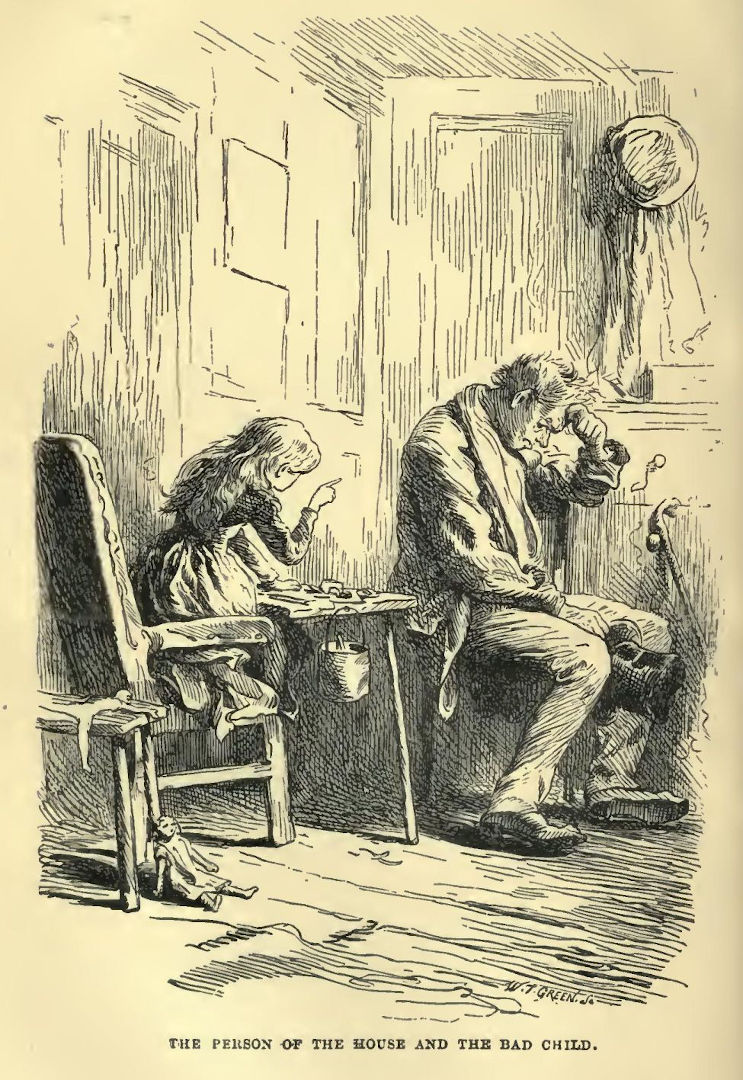
\includegraphics[scale=2.3]{02-02-01}

The shaking figure, unnerved and disjointed from head to foot, put
out its two hands a little way, as making overtures of peace and
reconciliation. Abject tears stood in its eyes, and stained the blotched
red of its cheeks. The swollen lead-coloured under lip trembled with a
shameful whine. The whole indecorous threadbare ruin, from the broken
shoes to the prematurely-grey scanty hair, grovelled. Not with any sense
worthy to be called a sense, of this dire reversal of the places of
parent and child, but in a pitiful expostulation to be let off from a
scolding.

‘I know your tricks and your manners,’ cried Miss Wren. ‘I know where
you’ve been to!’ (which indeed it did not require discernment to
discover). ‘Oh, you disgraceful old chap!’

The very breathing of the figure was contemptible, as it laboured and
rattled in that operation, like a blundering clock.

‘Slave, slave, slave, from morning to night,’ pursued the person of the
house, ‘and all for this! WHAT do you mean by it?’

There was something in that emphasized ‘What,’ which absurdly frightened
the figure. As often as the person of the house worked her way round to
it--even as soon as he saw that it was coming--he collapsed in an extra
degree.

‘I wish you had been taken up, and locked up,’ said the person of the
house. ‘I wish you had been poked into cells and black holes, and run
over by rats and spiders and beetles. I know their tricks and their
manners, and they’d have tickled you nicely. Ain’t you ashamed of
yourself?’

‘Yes, my dear,’ stammered the father.

‘Then,’ said the person of the house, terrifying him by a grand muster
of her spirits and forces before recurring to the emphatic word, ‘WHAT
do you mean by it?’

‘Circumstances over which had no control,’ was the miserable creature’s
plea in extenuation.

‘I’LL circumstance you and control you too,’ retorted the person of the
house, speaking with vehement sharpness, ‘if you talk in that way. I’ll
give you in charge to the police, and have you fined five shillings when
you can’t pay, and then I won’t pay the money for you, and you’ll be
transported for life. How should you like to be transported for life?’

‘Shouldn’t like it. Poor shattered invalid. Trouble nobody long,’ cried
the wretched figure.

‘Come, come!’ said the person of the house, tapping the table near her
in a business-like manner, and shaking her head and her chin; ‘you know
what you’ve got to do. Put down your money this instant.’

The obedient figure began to rummage in its pockets.

‘Spent a fortune out of your wages, I’ll be bound!’ said the person of
the house. ‘Put it here! All you’ve got left! Every farthing!’

Such a business as he made of collecting it from his dogs’-eared
pockets; of expecting it in this pocket, and not finding it; of not
expecting it in that pocket, and passing it over; of finding no pocket
where that other pocket ought to be!

‘Is this all?’ demanded the person of the house, when a confused heap of
pence and shillings lay on the table.

‘Got no more,’ was the rueful answer, with an accordant shake of the
head.

‘Let me make sure. You know what you’ve got to do. Turn all your pockets
inside out, and leave ‘em so!’ cried the person of the house.

He obeyed. And if anything could have made him look more abject or more
dismally ridiculous than before, it would have been his so displaying
himself.

‘Here’s but seven and eightpence halfpenny!’ exclaimed Miss Wren, after
reducing the heap to order. ‘Oh, you prodigal old son! Now you shall be
starved.’

‘No, don’t starve me,’ he urged, whimpering.

‘If you were treated as you ought to be,’ said Miss Wren, ‘you’d be fed
upon the skewers of cats’ meat;--only the skewers, after the cats had
had the meat. As it is, go to bed.’

When he stumbled out of the corner to comply, he again put out both his
hands, and pleaded: ‘Circumstances over which no control--’

‘Get along with you to bed!’ cried Miss Wren, snapping him up. ‘Don’t
speak to me. I’m not going to forgive you. Go to bed this moment!’

Seeing another emphatic ‘What’ upon its way, he evaded it by complying
and was heard to shuffle heavily up stairs, and shut his door, and throw
himself on his bed. Within a little while afterwards, Lizzie came down.

‘Shall we have our supper, Jenny dear?’

‘Ah! bless us and save us, we need have something to keep us going,’
returned Miss Jenny, shrugging her shoulders.

Lizzie laid a cloth upon the little bench (more handy for the person of
the house than an ordinary table), and put upon it such plain fare as
they were accustomed to have, and drew up a stool for herself.

‘Now for supper! What are you thinking of, Jenny darling?’

‘I was thinking,’ she returned, coming out of a deep study, ‘what I
would do to Him, if he should turn out a drunkard.’

‘Oh, but he won’t,’ said Lizzie. ‘You’ll take care of that, beforehand.’

‘I shall try to take care of it beforehand, but he might deceive me.
Oh, my dear, all those fellows with their tricks and their manners do
deceive!’ With the little fist in full action. ‘And if so, I tell you
what I think I’d do. When he was asleep, I’d make a spoon red hot, and
I’d have some boiling liquor bubbling in a saucepan, and I’d take it
out hissing, and I’d open his mouth with the other hand--or perhaps he’d
sleep with his mouth ready open--and I’d pour it down his throat, and
blister it and choke him.’

‘I am sure you would do no such horrible thing,’ said Lizzie.

‘Shouldn’t I? Well; perhaps I shouldn’t. But I should like to!’

‘I am equally sure you would not.’

‘Not even like to? Well, you generally know best. Only you haven’t
always lived among it as I have lived--and your back isn’t bad and your
legs are not queer.’

As they went on with their supper, Lizzie tried to bring her round to
that prettier and better state. But, the charm was broken. The person
of the house was the person of a house full of sordid shames and cares,
with an upper room in which that abased figure was infecting even
innocent sleep with sensual brutality and degradation. The doll’s
dressmaker had become a little quaint shrew; of the world, worldly; of
the earth, earthy.

Poor doll’s dressmaker! How often so dragged down by hands that should
have raised her up; how often so misdirected when losing her way on the
eternal road, and asking guidance! Poor, poor little doll’s dressmaker!



